\chapter{Analisis}
\label{chap: analisis}

Pada bab ini akan dibahas mengenai analisis sistem kini, analisis sistem usulan, dan use case diagram.

\section{Analisis Sistem Kini}
\label{sec: analisiSKini}

Skripsi 2 merupakan salah satu mata kuliah dengan syarat wajib lulus pada Program Studi Teknik Informatika Universitas Katolik Parahyangan, Bandung. Untuk mendapatkan hak sidang, mahasiswa wajib menempuh persyaratan-persyaratan yang sudah ditentukan pada kelas matakuliah Skripsi 2, yaitu mahasiswa harus melakukan proses bimbingan (disarankan 4 kali bimbingan), mahasiswa harus mengikuti seminar internal 3 kali, dan mahasiswa wajib menyelesaikan dokumen serta program skripsi yang dikerjakan sebelum tanggal pengumpulan yang telah ditentukan. Jika mahasiswa tidak menyelesaikan persyaratan-persyaratan tersebut, maka mahasiswa yang bersangkutan tidak mendapatkan hak untuk menempuh sidang Skripsi 2.

Sistem penilaian yang dipakai saat ini pada sidang Skripsi 2 adalah sistem pencatatan manual pada formulir penilaian. Formulir penilaian yang digunakan untuk sistem kini terbagi menjadi 2 bagian, yaitu formulir rekapitulasi penilaian dan formulir berita acara sidang skripsi. Berikut ini adalah penjelasan penggunaan kertas formulir tersebut.

	\subsection{Form Rekapitulasi Penilaian}
	\label{sub: rekapPenil}
	
	Formulir rekapitulasi dibagi menjadi 3 bagian (Gambar \ref{fig: rekapAsli}), yaitu:
		\begin{enumerate}
			\item Lembar Rekapitulasi Penilaian Pembimbing
			\item Lembar Rekapitulasi Penilaian Ketua Tim Penguji
			\item Lembar Rekapitulasi Penilaian Anggota Tim Penguji
		\end{enumerate}
	
	Lembaran tersebut akan diberikan kepada pembimbing, ketua tim penguji, dan anggota tim penguji sesuai dengan keperluannya. Setelah dibagikan, penilai wajib mengisi kolom nilai yang ingin diberikan kepada mahasiswa yang bersangkutan sesuai dengan kolom komponen penilaian yang ada. Setelah memberikan nilai, maka penilai harus melakukan perkalian antara kolom nilai dengan kolom bobot yang akan menghasilkan kolom nilai akhir mahasiswa. Terakhir penilai akan menjumlahkan seluruh kolom nilai akhir yang akan menghasilkan total nilai akhir dari mahasiswa tersebut.
	
	Setelah semua kolom terisi, maka lembaran rekapitulasi tersebut akan dikumpulkan ke ketua tim penguji. Kemudian data yang telah tersedia akan disalin oleh ketua tim penguji kepada formulir berita acara sidang skripsi.
	
	\subsection{Form Berita Acara Sidang Skripsi}
	\label{sub: formSkripsi}
	
	Formulir berita acara sidang skripsi (Gambar \ref{fig: skripsiAsli}) merupakan formulir yang mencakup pengisian waktu sidang bersangkutan, data diri mahasiswa, nama dosen penguji dan pembimbing, nilai akhir dari masing-masing penilai, dan nilai akhir yang diterima mahasiswa. Seperti yang telah dibahas pada subbab sebelumnya (\ref{sub: rekapPenil}) formulir berita acara sidang skripsi akan diisi oleh ketua tim penguji setelah seluruh form rekapitulasi dari masing masing penilai di kumpulkan kembali kepada ketua tim penguji.
	
	Setelah ketua tim penguji melakukan pengisian pada masing-masing kolom dari masing-masing penilai yang bersangkutan, maka ketua tim penguji akan melakukan perkalian nilai tersebut dengan bobot masing-masing penilai yang akan menghasilkan nilai akhir mahasiswa dari masing-masing penilai. Kemudian akan dihasilkan 90\% nilai akhir mahasiswa untuk diberitahukan kepada mahasiswa dan diberikan kepada koordinator skripsi untuk melengkapi 10\% dari nilai mahasiswa berdasarkan nilai kedisiplinan. Hasil dari seluruh proses tersebut adalah nilai akhir sidang skripsi 2 mahasiswa bersangkutan.
	
\section{Analisis Sistem Usulan}
\label{sec: analisisSUsulan}

Masalah yang dihadapi oleh sistem kini adalah tidak adanya otomatisasi dalam pengisian formulir penilaian. Tidak adanya otomatisasi pada sistem kini mengakibatkan kemungkinan dapat terjadinya \textit{human error} (kesalahan manusia yang tidak disengaja), sehingga data yang dihasilkan tidak valid.

Untuk menyelesaikan masalah tersebut, penulis memakai AngularJS sebagai solusi dalam otomatisasi formulir penilaian. Dengan memakai AngularJS, maka formulir penilaian sistem kini yang berupa kertas dapat digantikan dengan sistem penilaian berupa aplikasi berbasis \textit{web}. Gambar \ref{fig:flowchart} adalah \textit{flowchart} dari aplikasi berbasis \textit{web} yang akan dibangun.

\begin{figure}[H]
	\centering
	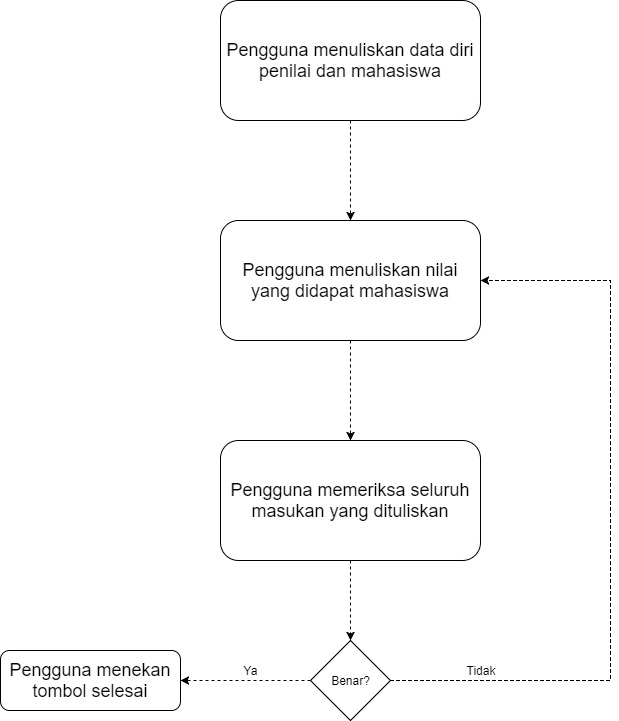
\includegraphics[scale=0.43]{Gambar/flowchart}
	\caption{Flowchart sistem usulan}
	\label{fig:flowchart}
\end{figure}

Sistem usulan yang akan dibuat adalah sebuah sistem berbasis \textit{web} menggunakan bahasa pemrograman PHP yang dapat melakukan otomatisasi perhitungan nilai akhir mahasiswa. Otomatisasi tersebut dilakukan dengan mengintegrasikan bahasa pemrograman AngularJS ke dalam bahasa PHP sehingga menghasilkan sistem penilaian yang bersifat Single Page Application. Sedangkan tampilan pada sistem usulan akan dibuat semirip mungkin dengan tampilan yang ada pada sistem kini, sehingga pengguna mudah untuk mempelajari sistem usulan yang dibuat.

Analisis sistem usulan dibagi menjadi beberapa tahap, yaitu analisis \textit{back end}, analisis \textit{front end}, dan analisis basis data. Berikut ini penjelasannya.
	
	\subsection{Analisis Back End}
	\label{sub: backEnd}
	
	Analisis tahap \textit{back end} merupakan analisis pada lapisan data akses dan kode-kode yang bekerja secara tidak terlihat pada suatu aplikasi. Pada sistem informasi penilaian sidang skripsi 2, analisis tahap ini membahas tentang pembuatan kode \textit{model, view, controller} dari \textit{codeigniter}. Berikut ini adalah penjelasan lengkapnya:
	
	\subsubsection{Model}
	\label{subsub: modelCI}
	
	Pada bagian ini akan dijelaskan tentang penggunaan \textit{model} pada \textit{codeigniter}. \textit{Model} mempunyai fungsi untuk membuat sambungan dari aplikasi ke basis data. Pada penelitian ini hanya memiliki 1 kelas diberi nama "Skripsi\_model" dengan format \textit{extends CI\_Model} yang berfungsi untuk mengaktifka fitur dari model milik codeigniter. Kelas model sendiri memiliki sebuah method yang dinamakan "InsertDataMahasiswa" dengan parameter \$tablename untuk masukan nama tabel dan \$data untuk masukan data yang diperoleh dari \textit{controller}. Method tersebut berfungsi untuk melakukan fungsi \textit{insert} ke dalam basis data sistem usulan.
	
	\subsubsection{Controller}
	\label{subsub: controllerCI}
	
	Pada bagian ini akan dijelaskan tentang kode dan kegunaannya pada kelas \textit{controller}. \textit{Controller} merupakan kelas yang mengatur hubungan antara kelas \textit{model} dan \textit{view} pada \textit{codeigniter}. Dengan memanfaatkan fungsi-fungsi dari \textit{codeigniter}, maka kelas \textit{controller} dapat dipersingkat dan dipermudah dalam pembuatannya.
	\begin{figure}[H]
		\centering
		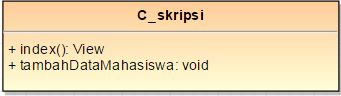
\includegraphics[scale= 1.0]{Gambar/C_skripsi}
		\caption {Gambar diagram kelas \textit{file controllers}}
		\label{fig:controllers}
	\end{figure}

	Berikut adalah \textit{method-method} yang dimiliki oleh kelas \textit{controller} Gambar \ref{fig:controllers}:
\begin{itemize}
	\item index()\\
	Berfungsi untuk memilih \textit{file view} yang akan dipakai pada sistem usulan.
	\item tambahDataMahasiswa\\
	Berfungsi untuk mengambil data yang telah terisi dari \textit{view} sistem dan mengubahnya menjadi \textit{compatible} sehingga dapat diproses kedalam \textit{method} insertDataMahasiswa pada kelas \textit{model} yang kemudian akan diproses ke dalam bahasa sql.
\end{itemize}
	
	\subsubsection{Helper}
	\label{sub: Helper}
	Helper merupakan salah satu fungsi dari codeigniter yang berguna untuk mempermudah pembuatan sistem usulan. Sistem usulan menggunakan dua buah helper yaitu \textit{helper url} agar sistem dapat memproses kode berupa \textit{url} untuk merujuk suatu halaman yang dituju, serta \textit{helper file} agar sistem dapat mengaktifkan fungsi-fungsi \textit{path} untuk merujuk \textit{file} yang dituju.
	
	\subsection{Analisis Front End}
	\label{sub: frontEnd}
	
	Analisis tahap \textit{front-end} merupakan analisis pada bagian yang akan ditampilkan kepada pengguna. Pada sistem usulan, analisis \textit{front-end} akan berfokus pada penggunaan AngularJS adalah otomatisasi perhitungan nilai akhir mahasiswa. 
	
	Tahap analisis \textit{front-end} adalah tahap seleksi masukan yang akan ditampilkan dan diisi oleh pengguna sistem. Diskusi dengan dosen pembimbing menghasilkan 28 buah masukan pada Tabel \ref{tabel: masukan} yang akan ditampilkan pada tampilan sistem usulan. 
	\begin{table}[H]
		\centering
		\caption{Tabel masukan pada tampilan}
		\label{tabel: masukan}
		\begin{tabular}{| m{0.75cm} | m{10cm} |}
			\hline
			No & Masukan\\
			\hline
			1 & Tahun Sidang\\
			\hline
			2 & Semester Sidang\\
			\hline
			3 & NPM\\
			\hline
			4 & Nama Mahasiswa\\
			\hline
			5 & Judul Skripsi\\
			\hline
			6 & Nama Pembimbing\\
			\hline
			7 & Nama Pembimbing Pendamping\\
			\hline
			8 & Nama Ketua Tim Penguji\\
			\hline
			9 & Nama Anggota Tim Penguji\\
			\hline
			10 & Nilai Ketua Tim Penguji\\
			\hline
			11 & Nilai Anggota Tim Penguji\\
			\hline
			12 & Nilai Pembimbing\\
			\hline
			13 & Nilai Koordinator Skripsi\\
			\hline
			14 & Nilai Koordinator Skripsi\\
			\hline
			15 & Nilai Tata Tulis Laporan Anggota\\
			\hline
			16 & Nilai Kelengkapan Materi Anggota\\
			\hline
			17 & Nilai Penguasaan Materi Anggota\\
			\hline
			18 & Nilai Presentasi Anggota\\
			\hline
			19 & Nilai Pencapaian Tujuan Anggota\\
			\hline
			20 & Nilai Tata Tulis Laporan Ketua\\
			\hline
			21 & Nilai Kelengkapan Materi Ketua\\
			\hline
			22 & Nilai Penguasaan Materi Ketua\\
			\hline
			23 & Nilai Presentasi Ketua\\
			\hline
			24 & Nilai Pencapaian Tujuan Ketua\\
			\hline
			25 & Nilai Tata Tulis Laporan Pembimbing\\
			\hline
			26 & Nilai Kelengkapan Materi Pembimbing\\
			\hline
			27 & Nilai Penguasaan Materi Pembimbing\\
			\hline
			28 & Proses Bimbingan\\
			\hline
		\end{tabular}
	\end{table}

	Berdasarkan masukan pada Tabel \ref{tabel: masukan}, dibuatlah \textit{Model, View, Controller} bagian \textit{front-end} yang akan dipakai oleh AngularJS sebagai cara otomatisasi sistem. Masukan-masukan yang dibuat akan diberikan variabel ng-model sebagai tempat penyimpanan masukan untuk diberikan pada \textit{view} dari AngularJS sehingga otomatisasi dapat terjadi.
	
	\textit{View} pada AngularJS akan memanggil masukan pada \textit{model} dan melakukan otomatisasi, baik perhitungan atau pengisian otomatis. Sementara \textit{controller} dibuat pada awal kode sistem, agar \textit{view} dan \textit{model} sistem dapat terhubung satu dengan yang lain.
	
	Berikut ini adalah nama-nama dari \textit{model, view,} dan \textit{controller} AngularJS yang dipakai untuk otomatisasi pada Sistem Penilaian Sidang Skripsi 2.
	\begin{itemize}
		\item \textit{Controller}: "DefaultValue" = Controller yang dipakai di seluruh sistem
		\item \textit{Model}:\\
		\begin{table}[H]
			\centering
			\caption{Tabel model}
			\label{tabel: model}
		\begin{tabular}{| m{5cm} | m{10cm} |}
			\hline
			Nama Model & Tujuan\\
			\hline
			 tahun & Masukan Tahun\\
			\hline
			 n\_npm & Masukan NPM\\
			\hline
			namaPembimbing & Masukan nama pembimbing\\
			\hline
			namaKetuaTimPenguji & Masukan nama ketua tim penguji\\
			\hline
			namaAnggotaTimPenguji & Masukan nama anggota tim penguji\\
			\hline
			 nilai\_koordinator & Masukan nilai Koordinator skripsi\\
			 \hline
			 koordinator.value & Bobot nilai koordinator skripsi\\
			\hline
			 nilai\_TTLaporanK & Masukan nilai tata tulis laporan milik ketua tim penguji\\
			 \hline
			 TTLaporanK.value & Bobot nilai tata tulis laporan milik ketua tim penguji\\
			\hline
			 nilai\_KMateriK & Masukan nilai kelengkapan materi milik ketua tim penguji\\
			\hline
			 KMateriK.value & Bobot nilai kelengkapan materi milik ketua tim penguji\\
			 \hline
			 nilai\_PMateriK & Masukan nilai penguasaan materi milik ketua tim penguji\\
			 \hline
			 PMateriK.value & Bobot nilai penguasaan materi milik ketua tim penguji\\
			\hline
			 nilai\_presentasiK& Masukan nilai presentasi ketua tim penguji\\
			 \hline
			 presentasiK.value & Bobot nilai presentasi ketua tim penguji\\
			\hline
			 nilai\_PTujuanK & Masukan nilai pecapaian tujuan milik ketua tim penguji\\
			\hline
			PTujuanK.value & Bobot nilai pecapaian tujuan milik ketua tim penguji\\
			\hline
			 nilai\_TTLaporanA & Masukan nilai tata tulis laporan milik anggota tim penguji\\
			\hline
			TTLaporanA.value & Bobot nilai tata tulis laporan milik anggota tim penguji\\
			\hline
			 nilai\_KMateriA & Masukan nilai kelengkapan materi milik anggota tim penguji\\
			 \hline
			 KMateriA.value & Bobot nilai kelengkapan materi milik anggota tim penguji\\
			\hline
			 nilai\_PMateriA & Masukan nilai penguasaan materi milik anggota tim penguji\\
			\hline
			PMateriA.value & Bobot nilai penguasaan materi milik anggota tim penguji\\
			\hline
			 nilai\_presentasiA & Masukan nilai presentasi milik anggota tim penguji\\
			\hline
			presentasiA.value & Bobot nilai presentasi milik anggota tim penguji\\
			\hline
			 nilai\_PTujuanA & Masukan nilai pencapaian tujuan milik anggota tim penguji\\
			 \hline
			 PTujuanA.value & Bobot nilai pencapaian tujuan milik anggota tim penguji\\
			\hline
			 nilai\_TTLaporanP & Masukan nilai tata tulis laporan milik pembimbing\\
			\hline
			TTLaporanP.value & Bobot nilai tata tulis laporan milik pembimbing\\
			\hline
			 nilai\_KMateriP & Masukan nilai kelengkapan materi milik pembimbing\\
			 \hline
			 KMateriP.value & Bobot nilai kelengkapan materi milik pembimbing\\
			\hline
			 nilai\_PMateriP & Masukan nilai penguasaan materi milik pembimbing\\
			 \hline
			 PMateriP.value & Bobot nilai penguasaan materi milik pembimbing\\
			\hline
			 nilai\_PBimbinganP & Masukan nilai proses bimbingan milik pembimbing\\
			\hline
			PBimbinganP.value & Bobot ilai proses bimbingan milik pembimbing\\
			\hline
		\end{tabular}
	\end{table}
		\item View:
		\begin{table}[H]
			\centering
			\caption{Tabel view}
			\label{tabel: view}
			\begin{tabular}{| m{5cm} | m{10cm} |}
				\hline
				Otomatisasi view & Keterangan\\
				\hline
				Tahun+1 & mengambil masukan model "tahun" ditambah 1\\
				\hline
				NPM & mengambil masukan model "npm" dan menampilkan isinya di lembaran rekapitulasi\\
				\hline
				Nilai ketua tim penguji & mengambil total nilai akhir dari lembar rekapitulasi ketua tim penguji\\
				\hline
				Nilai anggota tim penguji & mengambil total nilai akhir dari lembar rekapitulasi anggota tim penguji\\
				\hline
				Nilai pembimbing & mengambil total nilai akhir dari lembar rekapitulasi pembimbing\\
				\hline
				Nilai akhir ketua tim penguji & mengambil nilai ketua tim penguji dan dikalikan dengan bobot nilai ketua tim penguji\\
				\hline
				Nilai akhir anggota tim penguji & mengambil nilai anggota tim penguji dan dikalikan dengan bobot anggota ketua tim penguji\\
				\hline
				Nilai akhir pembimbing & mengambil nilai pembimbing dan dikalikan dengan bobot nilai pembimbing\\
				\hline
				Nilai akhir koordinator skripsi & mengambil nilai koordinator skripsi dan dikalikan dengan bobot nilai koordinator skripsi\\
				\hline
				Nilai akhir tata tulis laporan ketua tim penguji & mengambil nilai tata tulis laporan ketua tim penguji dan dikalikan dengan bobot nilai tata tulis laporan ketua tim penguji\\
				\hline
				Nilai akhir kelengkapan materi ketua tim penguji & mengambil nilai kelengkapan materi ketua tim penguji dan dikalikan dengan bobot nilai kelengkapan materi ketua tim penguji\\
				\hline
				Nilai akhir penguasaan materi ketua tim penguji & mengambil nilai penguasaan materi ketua tim penguji dan dikalikan dengan bobot nilai penguasaan materi ketua tim penguji\\
				\hline
				Nilai akhir presentasi ketua tim penguji & mengambil nilai presentasi ketua tim penguji dan dikalikan dengan bobot nilai presentasi ketua tim penguji\\
				\hline
				Nilai akhir pencapaian tujuan ketua tim penguji & mengambil nilai pencapaian tujuan ketua tim penguji dan dikalikan dengan bobot nilai pencapaian tujuan ketua tim penguji\\
				\hline
				Total nilai akhir ketua tim penguji & menjumlahkan seluruh nilai akhir ketua tim penguji pada lembar rekapitulasi ketua tim penguji\\
				\hline
				Nilai akhir tata tulis laporan anggota tim penguji & mengambil nilai tata tulis laporan anggota tim penguji dan dikalikan dengan bobot nilai tata tulis laporan anggota tim penguji\\
				\hline
				Nilai akhir kelengkapan materi anggota tim penguji & mengambil nilai kelengkapan materi anggota tim penguji dan dikalikan dengan bobot nilai kelengkapan materi anggota tim penguji\\
				\hline
				Nilai akhir penguasaan materi anggota tim penguji & mengambil nilai penguasaan materi anggota tim penguji dan dikalikan dengan bobot nilai penguasaan materi anggota tim penguji\\
				\hline
				Nilai akhir presentasi anggota tim penguji & mengambil nilai presentasi anggota tim penguji dan dikalikan dengan bobot nilai presentasi anggota tim penguji\\
				\hline
				Nilai akhir pencapaian tujuan anggota tim penguji & mengambil nilai pencapaian tujuan anggota tim penguji dan dikalikan dengan bobot nilai pencapaian tujuan anggota tim penguji\\
				\hline
				Total nilai akhir anggota tim penguji & menjumlahkan seluruh nilai akhir anggota tim penguji pada lembar rekapitulasi anggota tim penguji\\
				\hline
				Nilai akhir tata tulis laporan pembimbing & mengambil nilai tata tulis laporan pembimbing dan dikalikan dengan bobot nilai tata tulis laporan pembimbing\\
				\hline
				Nilai akhir kelengkapan materi pembimbing & mengambil nilai kelengkapan materi pembimbing dan dikalikan dengan bobot nilai kelengkapan materi pembimbing\\
				\hline
			\end{tabular}
		\end{table}
		\begin{table}
			\centering
			\begin{tabular}{| m{5cm} | m{10cm} |}
				\hline
				Nilai akhir penguasaan materi pembimbing & mengambil nilai penguasaan materi pembimbing dan dikalikan dengan bobot nilai penguasaan materi pembimbing\\
				\hline
				Nilai akhir proses bimbingan pembimbing & mengambil nilai proses bimbingan pembimbing dan dikalikan dengan bobot nilai proses bimbingan pembimbing\\
				\hline
				Total nilai akhir pembimbing & menjumlahkan seluruh nilai akhir pembimbing pada lembar rekapitulasi pembimbing\\
				\hline
				Persetujuan ketua tim penguji & menampilkan model namaKetuaTimPenguji\\
				\hline
				Persetujuan anggota tim penguji & menampilkan model namaAnggotaTimPenguji\\
				\hline
				Persetujuan pembimbing & menampilkan model namaPembimbing\\
				\hline
			\end{tabular}
		\end{table}
	\end{itemize}
	
	\subsection{Analisis Basis Data}
	\label{sub: analisisDatabase}
	
	Sistem Informasi Penilaian Sidang Skripsi 2 menggunakan perangkat lunak mysql sebagai sarana penyimpanan dan pengolahan basis data. Didalam \textit{folder} "application" terdapat \textit{folder} "models" yang berfungsi menghubungkan basis data dengan sistem. 
	
	Berdasarkan analisa dari contoh form penilaian skripsi yang ada (Gambar \ref{fig: skripsiAsli} dan Gambar \ref{fig: rekapAsli}), dapat disimpulkan bahwa penilaian skripsi membutuhkan data-data sebagai berikut:
		
		\begin{enumerate}
			\item Semester
			\item Tahun ajaran
			\item NPM mahasiswa 
			\item Nama mahasiswa
			\item Judul skripsi
			\item Nama pembimbing utama/tunggal
			\item Nama pembimbing pendamping(tidak harus)
			\item Nama ketua tim penguji
			\item Nama anggota tim penguji
			\item Bobot ketua tim penguji
			\item Bobot anggota tim penguji
			\item Bobot pembimbing
			\item Nilai koordinator skripsi
			\item Bobot koordinator skripsi
			\item Bobot tata tulis laporan ketua
			\item Bobot kelengkapan materi ketua
			\item Bobot penguasaan materi ketua
			\item Bobot presentasi ketua
			\item Bobot pencapaian tujuan ketua
			\item Bobot tata tulis laporan anggota
			\item Bobot kelengkapan materi anggota
			\item Bobot penguasaan materi anggota
			\item Bobot presentasi anggota
			\item Bobot pencapaian tujuan anggota
			\item Bobot tata tulis laporan pembimbing
			\item Bobot kelengkapan materi pembimbing
			\item Bobot penguasaan materi pembimbing
			\item Bobot bimbingan pembimbing
			\item Nilai akhir mahasiswa
		\end{enumerate}
	
	Berdasarkan diskusi dengan dosen pembimbing, disimpulkan bahwa sistem penilaian sidang skripsi 2 ini hanya memerlukan penyimpanan untuk bobot masing-masing penilaian dan nilai akhir mahasiswa untuk tahap perhitungan. Hal ini dikarenakan nilai-nilai lainnya dapat dihasilkan dengan melakukan perhitungan pada  nilai akhir mahasiswa dan bobot nilai yang diinginkan. Begitu pula dengan nilai dari masing-masing penguji.
	
\section{Use Case}
\label{sec: usecaseDiagram}

	\begin{figure}[H]
		\centering
		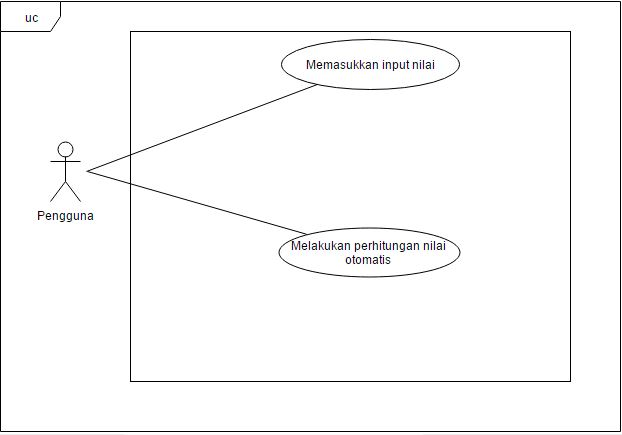
\includegraphics[scale=0.75]{Gambar/usecase}
		\caption{Use case diagram}
		\label{fig:usecase}
	\end{figure}
	
	\begin{enumerate}
		\item Skenario memasukkan nilai\\
			Deskripsi: Kegiatan memasukkan nilai ke dalam kotak input yang ada.\\
			Aktor: Ketua tim penguji\\
			Prakondisi: - \\
			Skenario:
			\begin{itemize}
				\item Pengguna memilih tempat/kolom yang sudah tersedia di tampilan
				\item Pengguna memasukkan nilai yang diinginkan pada tempat/kolom yang telah dipilih.
			\end{itemize}
		\item Skenario melakukan perhitungan otomatis\\
			Deskripsi: Melakukan perhitungan secara otomatis pada tampilan\\
			Aktor: -\\
			Prakondisi: Nilai sudah dimasukkan\\
			Skenario:
			\begin{itemize}
				\item Pengguna mengisi kolom nilai yang sudah disediakan
				\item Dengan ng-model, sistem mengambil nilai dari tempat/kolom yang sudah diisi dan melakukan perhitungan
				\item Sistem menampilkan hasil perhitungan ke dalam kolom yang disediakan untuk hasil perhitungan.
			\end{itemize}
	\end{enumerate}
	